
%(BEGIN_QUESTION)
% Copyright 2006, Tony R. Kuphaldt, released under the Creative Commons Attribution License (v 1.0)
% This means you may do almost anything with this work of mine, so long as you give me proper credit

Determine the following test point voltages (all with reference to ground) at the following temperatures, for the following 4-wire RTD circuit:

$$\includegraphics[width=15.5cm]{i00652x01.eps}$$

\begin{itemize}
\item{} Voltage at TP1 ($V_{TP1}$), with RTD at 0$^{o}$ C = \underbar{\hskip 50pt} V
\vskip 5pt
\item{} Voltage at TP2 ($V_{TP2}$), with RTD at 10$^{o}$ F = \underbar{\hskip 50pt} V
\vskip 5pt
\item{} Voltage at TP3 ($V_{TP3}$), with RTD at 12$^{o}$ C = \underbar{\hskip 50pt} V
\vskip 5pt
\item{} Voltage at TP5 ($V_{TP5}$), with RTD at -20$^{o}$ C = \underbar{\hskip 50pt} V
\end{itemize}

\underbar{file i00652}
%(END_QUESTION)





%(BEGIN_ANSWER)

Remember these simplifying assumptions of negative feedback opamp circuits:

\begin{itemize}
\item{} Negative feedback will force the output voltage to whatever value is necessary to maintain the differential input voltage at zero.
\item{} Input terminals on the opamp(s) draw negligible current.
\end{itemize}

Voltages at TP1 and TP2 (with reference to ground) may be calculated simply by evaluating voltage drops in the series RTD circuit.  Voltage at TP3 with reference to ground will be identical to that at TP1, since the upper opamp simply functions as a voltage follower.  TP5 is the output of this differential amplifier circuit, representing the difference between potentials sensed at inputs TP1 and TP2 (i.e. the voltage dropped by the RTD).  The reason why the output voltage is a negative quantity (with respect to ground) is because the differential amplifier's noninverting input sees a lower voltage than its inverting input.

\vskip 10pt

For each of the voltage calculations, you will need to reference an RTD table to find the proper RTD resistance values.  While it is possible to use a formula to approximate RTD resistance based on temperature, a table will give you more accurate answers because a table accounts for all nonlinearities of the RTD, while the formula assumes a perfectly linear characteristic.

\vskip 10pt

\begin{itemize}
\item{} Voltage at TP1 ($V_{TP1}$), with RTD at 0$^{o}$ C ($R_{RTD}$ = 100.0 $\Omega$) = \underbar{\bf 0.1524} V
\vskip 5pt
\item{} Voltage at TP2 ($V_{TP2}$), with RTD at 10$^{o}$ F ($R_{RTD}$ = 95.21 $\Omega$) = \underbar{\bf 0.0024} V ({\bf 2.4} mV)
\vskip 5pt
\item{} Voltage at TP3 ($V_{TP3}$), with RTD at 12$^{o}$ C ($R_{RTD}$ = 104.68 $\Omega$) = \underbar{\bf 0.1594} V
\vskip 5pt
\item{} Voltage at TP5 ($V_{TP5}$), with RTD at -20$^{o}$ C ($R_{RTD}$ = 92.16 $\Omega$) = \underbar{\bf -0.1382} V
\end{itemize}

%(END_ANSWER)





%(BEGIN_NOTES)


%INDEX% Measurement, temperature: RTD (4-wire with cable resistance)

%(END_NOTES)


